% === Figure: CTA granularity-offset diagnostic ============================
% CONFIRMED numbers (offset of majority-direct type vs gold):
%   65.6% exact match ; 27.6% gold is a strict ANCESTOR (direct type too specific) ;
%   0.2% gold is finer ; 6.6% off-path.
% This reframes CTA as a granularity-SELECTION problem, not a reachability problem
%   (gold is reachable 97% of the time within a 4-hop P31 closure).
% Standalone-includable: % === Figure: CTA granularity-offset diagnostic ============================
% CONFIRMED numbers (offset of majority-direct type vs gold):
%   65.6% exact match ; 27.6% gold is a strict ANCESTOR (direct type too specific) ;
%   0.2% gold is finer ; 6.6% off-path.
% This reframes CTA as a granularity-SELECTION problem, not a reachability problem
%   (gold is reachable 97% of the time within a 4-hop P31 closure).
% Standalone-includable: % === Figure: CTA granularity-offset diagnostic ============================
% CONFIRMED numbers (offset of majority-direct type vs gold):
%   65.6% exact match ; 27.6% gold is a strict ANCESTOR (direct type too specific) ;
%   0.2% gold is finer ; 6.6% off-path.
% This reframes CTA as a granularity-SELECTION problem, not a reachability problem
%   (gold is reachable 97% of the time within a 4-hop P31 closure).
% Standalone-includable: % === Figure: CTA granularity-offset diagnostic ============================
% CONFIRMED numbers (offset of majority-direct type vs gold):
%   65.6% exact match ; 27.6% gold is a strict ANCESTOR (direct type too specific) ;
%   0.2% gold is finer ; 6.6% off-path.
% This reframes CTA as a granularity-SELECTION problem, not a reachability problem
%   (gold is reachable 97% of the time within a 4-hop P31 closure).
% Standalone-includable: \input{figures/cta_offset.tex} inside a figure env.
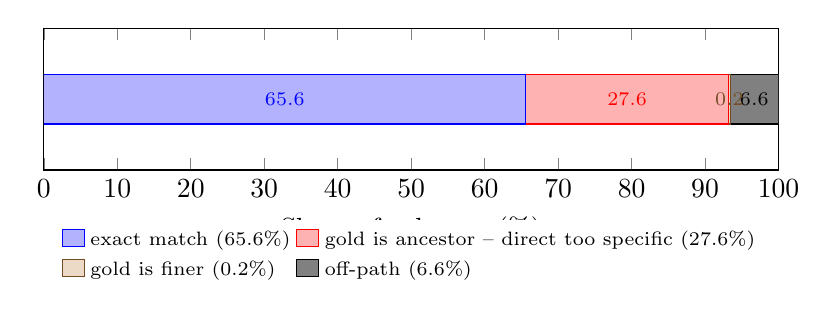
\begin{tikzpicture}
\begin{axis}[
    width=0.9\linewidth, height=4.2cm,
    xbar stacked,
    xmin=0, xmax=100,
    y=0.9cm,
    xlabel={Share of columns (\%)},
    ytick=\empty,
    bar width=18pt,
    nodes near coords,
    every node near coord/.append style={font=\scriptsize},
    legend style={at={(0.5,-0.35)}, anchor=north, legend columns=2, font=\scriptsize, draw=none},
    legend cell align=left,
]
% single stacked bar: each segment = one offset class (CONFIRMED).
\addplot+[xbar] coordinates {(65.6,0)};  \addlegendentry{exact match (65.6\%)}
\addplot+[xbar] coordinates {(27.6,0)};  \addlegendentry{gold is ancestor -- direct too specific (27.6\%)}
\addplot+[xbar] coordinates {(0.2,0)};   \addlegendentry{gold is finer (0.2\%)}
\addplot+[xbar] coordinates {(6.6,0)};   \addlegendentry{off-path (6.6\%)}
\end{axis}
\end{tikzpicture}

% Caption guidance (place when included): the dominant error mode is the
% majority-direct type being TOO SPECIFIC (27.6% of columns need to climb to an
% ancestor), with only 6.6% genuinely off-path. Hence the task is granularity
% SELECTION, not reachability -- exactly what FLINT's learned ranker addresses.
 inside a figure env.
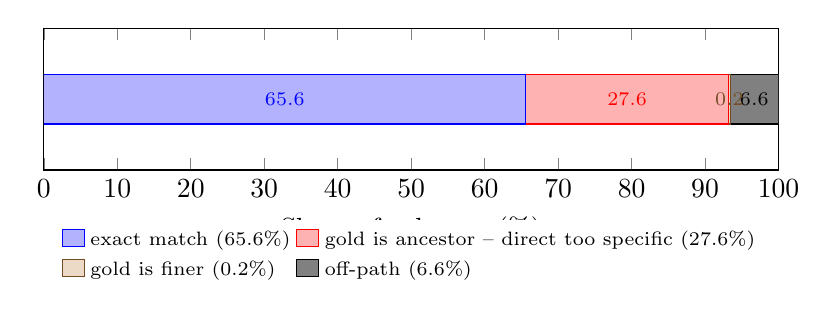
\begin{tikzpicture}
\begin{axis}[
    width=0.9\linewidth, height=4.2cm,
    xbar stacked,
    xmin=0, xmax=100,
    y=0.9cm,
    xlabel={Share of columns (\%)},
    ytick=\empty,
    bar width=18pt,
    nodes near coords,
    every node near coord/.append style={font=\scriptsize},
    legend style={at={(0.5,-0.35)}, anchor=north, legend columns=2, font=\scriptsize, draw=none},
    legend cell align=left,
]
% single stacked bar: each segment = one offset class (CONFIRMED).
\addplot+[xbar] coordinates {(65.6,0)};  \addlegendentry{exact match (65.6\%)}
\addplot+[xbar] coordinates {(27.6,0)};  \addlegendentry{gold is ancestor -- direct too specific (27.6\%)}
\addplot+[xbar] coordinates {(0.2,0)};   \addlegendentry{gold is finer (0.2\%)}
\addplot+[xbar] coordinates {(6.6,0)};   \addlegendentry{off-path (6.6\%)}
\end{axis}
\end{tikzpicture}

% Caption guidance (place when included): the dominant error mode is the
% majority-direct type being TOO SPECIFIC (27.6% of columns need to climb to an
% ancestor), with only 6.6% genuinely off-path. Hence the task is granularity
% SELECTION, not reachability -- exactly what FLINT's learned ranker addresses.
 inside a figure env.
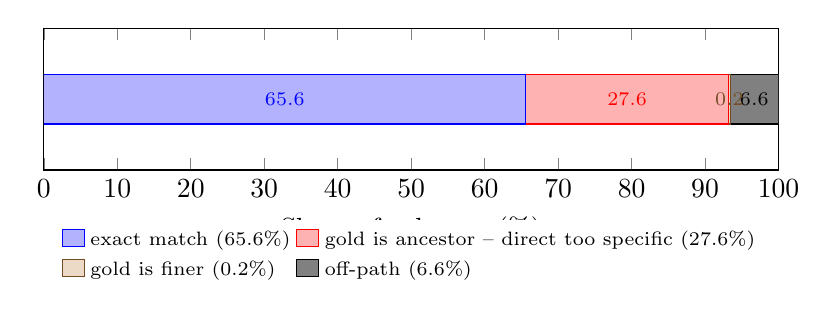
\begin{tikzpicture}
\begin{axis}[
    width=0.9\linewidth, height=4.2cm,
    xbar stacked,
    xmin=0, xmax=100,
    y=0.9cm,
    xlabel={Share of columns (\%)},
    ytick=\empty,
    bar width=18pt,
    nodes near coords,
    every node near coord/.append style={font=\scriptsize},
    legend style={at={(0.5,-0.35)}, anchor=north, legend columns=2, font=\scriptsize, draw=none},
    legend cell align=left,
]
% single stacked bar: each segment = one offset class (CONFIRMED).
\addplot+[xbar] coordinates {(65.6,0)};  \addlegendentry{exact match (65.6\%)}
\addplot+[xbar] coordinates {(27.6,0)};  \addlegendentry{gold is ancestor -- direct too specific (27.6\%)}
\addplot+[xbar] coordinates {(0.2,0)};   \addlegendentry{gold is finer (0.2\%)}
\addplot+[xbar] coordinates {(6.6,0)};   \addlegendentry{off-path (6.6\%)}
\end{axis}
\end{tikzpicture}

% Caption guidance (place when included): the dominant error mode is the
% majority-direct type being TOO SPECIFIC (27.6% of columns need to climb to an
% ancestor), with only 6.6% genuinely off-path. Hence the task is granularity
% SELECTION, not reachability -- exactly what FLINT's learned ranker addresses.
 inside a figure env.
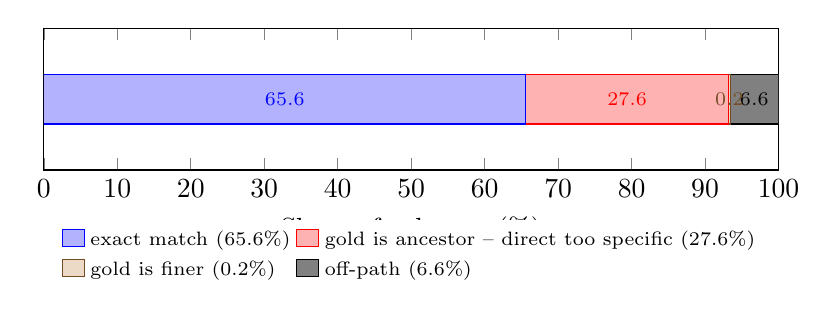
\begin{tikzpicture}
\begin{axis}[
    width=0.9\linewidth, height=4.2cm,
    xbar stacked,
    xmin=0, xmax=100,
    y=0.9cm,
    xlabel={Share of columns (\%)},
    ytick=\empty,
    bar width=18pt,
    nodes near coords,
    every node near coord/.append style={font=\scriptsize},
    legend style={at={(0.5,-0.35)}, anchor=north, legend columns=2, font=\scriptsize, draw=none},
    legend cell align=left,
]
% single stacked bar: each segment = one offset class (CONFIRMED).
\addplot+[xbar] coordinates {(65.6,0)};  \addlegendentry{exact match (65.6\%)}
\addplot+[xbar] coordinates {(27.6,0)};  \addlegendentry{gold is ancestor -- direct too specific (27.6\%)}
\addplot+[xbar] coordinates {(0.2,0)};   \addlegendentry{gold is finer (0.2\%)}
\addplot+[xbar] coordinates {(6.6,0)};   \addlegendentry{off-path (6.6\%)}
\end{axis}
\end{tikzpicture}

% Caption guidance (place when included): the dominant error mode is the
% majority-direct type being TOO SPECIFIC (27.6% of columns need to climb to an
% ancestor), with only 6.6% genuinely off-path. Hence the task is granularity
% SELECTION, not reachability -- exactly what FLINT's learned ranker addresses.
